% Faithful native paths from source/普通高考/2009/2009辽宁文.pdf, page 2.
% Original outlines, connected rock fissures, solid/dashed edges and shaded regions retained.
% Labels retain their original objects; no arbitrary geometric substitute or raster wrapper.
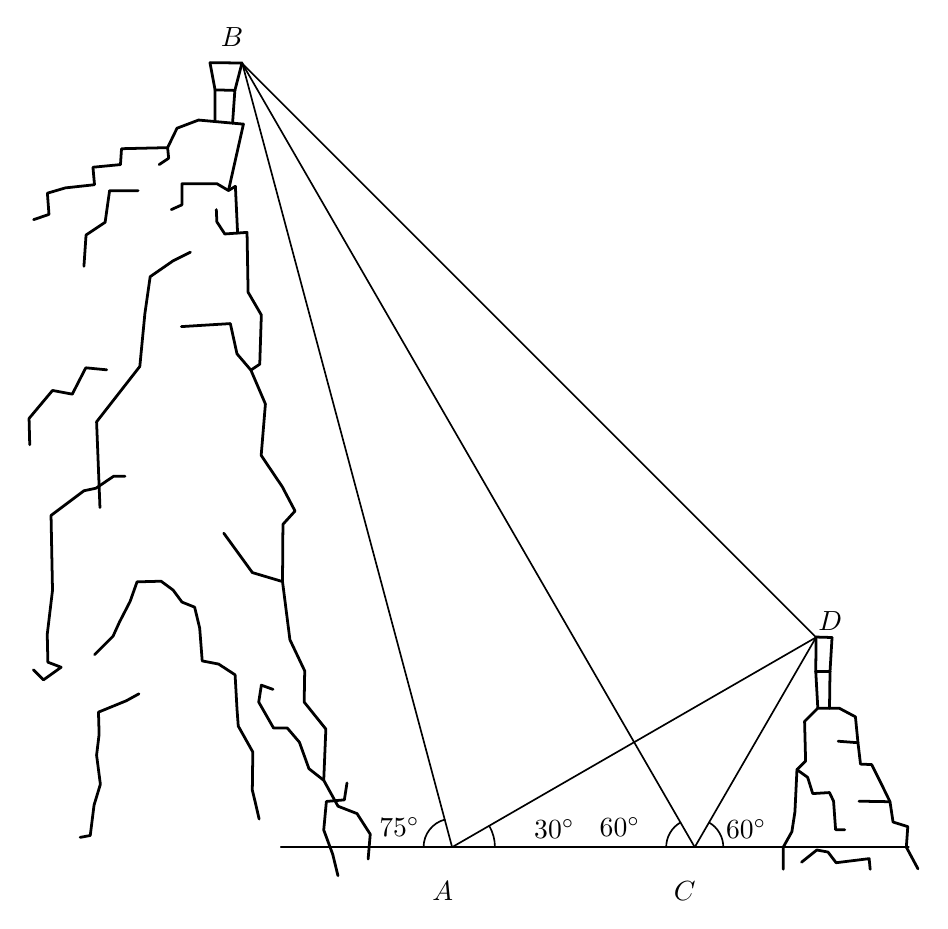
\begin{tikzpicture}[x=1cm,y=1cm,font=\normalsize,line join=round,line cap=round]
\path[draw=black,line width=0.6pt] (3.66030,1.11781) -- (11.63539,1.11781) ;
\path[draw=black,line width=0.6pt] (5.83533,1.11781) -- (3.17091,11.06858) ;
\path[draw=black,line width=0.6pt] (3.17091,11.06858) -- (10.45726,3.78223) ;
\path[draw=black,line width=0.6pt] (10.45726,3.78223) -- (8.91660,1.11781) ;
\path[draw=black,line width=0.6pt] (8.91660,1.11781) -- (3.17091,11.06858) ;
\path[draw=black,line width=0.6pt] (10.45726,3.78223) -- (5.83533,1.11781) ;
\path[draw=black,line width=1.0pt] (1.11111,1.24196) -- (1.23962,1.26605) -- (1.28784,1.65165) -- (1.36815,1.91671) -- (1.31997,2.28624) -- (1.35209,2.55132) -- (1.34406,2.83246) -- (1.69752,2.97705) -- (1.85815,3.06541) ;
\path[draw=black,line width=1.0pt] (3.38442,1.47493) -- (3.33621,1.68376) -- (3.29780,1.84281) -- (3.30408,2.32639) -- (3.11934,2.65576) -- (3.10326,2.87265) -- (3.07915,3.30641) -- (2.87031,3.44296) -- (2.66144,3.48315) -- (2.62931,3.90085) -- (2.56506,4.16594) -- (2.40440,4.23019) -- (2.29195,4.38283) -- (2.13931,4.49528) -- (1.83406,4.48725) -- (1.74570,4.23824) -- (1.60915,3.97314) -- (1.52881,3.79641) -- (1.29586,3.56346) ;
\path[draw=black,line width=1.0pt] (0.51667,3.37066) -- (0.64520,3.24214) -- (0.87011,3.40280) -- (0.70142,3.46707) -- (0.69341,3.82050) -- (0.76025,4.38036) -- (0.74159,5.33071) -- (1.15931,5.64398) -- (1.31193,5.67611) -- (1.53686,5.82873) -- (1.68145,5.82873) ;
\path[draw=black,line width=1.0pt] (0.47101,6.22781) -- (0.46245,6.56232) -- (0.76025,6.91789) -- (1.01135,6.87109) -- (1.18288,7.20557) -- (1.44877,7.17985) ;
\path[draw=black,line width=1.0pt] (1.36297,5.43019) -- (1.32011,6.51943) -- (1.86902,7.22271) -- (1.93369,7.89564) -- (2.00039,8.36262) -- (2.28949,8.56278) -- (2.51185,8.67396) ;
\path[draw=black,line width=1.0pt] (4.38530,0.75531) -- (4.31895,1.02713) -- (4.20484,1.33589) -- (4.23841,1.69834) -- (4.46664,1.71850) -- (4.50019,1.93328) ;
\path[draw=black,line width=1.0pt] (4.76867,0.96670) -- (4.79554,1.28218) -- (4.62771,1.54395) -- (4.38607,1.63794) -- (4.20484,1.96683) -- (4.01691,2.11451) -- (3.89607,2.45012) -- (3.74170,2.63134) -- (3.56719,2.63134) -- (3.37925,2.96026) -- (3.41280,3.17505) -- (3.56046,3.12134) ;
\path[draw=black,line width=1.0pt] (4.20484,1.96683) -- (4.23169,2.61792) -- (3.95650,2.96026) -- (3.96320,3.35629) -- (3.77528,3.75230) -- (3.68129,4.49066) -- (3.29869,4.60474) -- (2.93530,5.10536) ;
\path[draw=black,line width=1.0pt] (3.68129,4.49066) -- (3.68680,5.21784) -- (3.84037,5.38676) -- (3.67914,5.69390) -- (3.41040,6.09317) -- (3.46413,6.74586) -- (3.27985,7.17584) -- (3.10324,7.38315) -- (3.01878,7.76706) -- (2.39682,7.72868) ;
\path[draw=black,line width=1.0pt] (1.15931,8.49501) -- (1.18623,8.89181) -- (1.42834,9.05321) -- (1.48528,9.45542) -- (1.84778,9.45542) ;
\path[draw=black,line width=1.0pt] (3.27985,7.17584) -- (3.39222,7.25076) -- (3.41239,7.87625) -- (3.24426,8.16545) -- (3.23081,8.92544) -- (2.94833,8.90527) -- (2.84744,9.05996) -- (2.84071,9.21465) ;
\path[draw=black,line width=1.0pt] (3.11084,8.91686) -- (3.08285,9.51057) -- (2.99540,9.45676) -- (2.84744,9.54421) -- (2.40358,9.54421) -- (2.40358,9.27516) -- (2.26905,9.21465) ;
\path[draw=black,line width=1.0pt] (0.52039,9.08685) -- (0.71542,9.15411) -- (0.69526,9.42313) -- (0.92392,9.49039) -- (1.29384,9.53074) -- (1.27365,9.75269) -- (1.62340,9.78631) -- (1.63684,9.98808) -- (2.22198,10.00154) -- (2.23541,9.86702) -- (2.11436,9.78631) ;
\path[draw=black,line width=1.0pt] (2.22198,10.00154) -- (2.34167,10.24838) -- (2.61543,10.35195) -- (3.18507,10.30015) -- (2.99540,9.45676) ;
\path[draw=black,line width=1.0pt] (3.16685,11.07670) -- (2.76008,11.08030) ;
\path[draw=black,line width=1.0pt] (2.76008,11.08030) -- (2.82472,10.73541) ;
\path[draw=black,line width=1.0pt] (2.82472,10.73541) -- (3.07621,10.72823) ;
\path[draw=black,line width=1.0pt] (3.07621,10.72823) -- (3.16685,11.07670) ;
\path[draw=black,line width=1.0pt] (2.82472,10.73541) -- (2.82344,10.33304) ;
\path[draw=black,line width=1.0pt] (3.07621,10.72823) -- (3.04695,10.31271) ;
\path[draw=black,line width=1.0pt] (10.27287,0.92669) -- (10.46658,1.08164) -- (10.60860,1.05581) -- (10.71193,0.92021) -- (11.13159,0.97187) -- (11.14450,0.83630) ;
\path[draw=black,line width=1.0pt] (10.04044,0.83630) -- (10.04044,1.11781) -- (10.15021,1.31406) -- (10.18894,1.56586) -- (10.21476,2.10174) -- (10.35036,2.00491) -- (10.41491,1.79829) -- (10.62799,1.81120) -- (10.67962,1.70146) -- (10.70545,1.33990) -- (10.82166,1.33990) ;
\path[draw=black,line width=1.0pt] (11.75141,0.84274) -- (11.60380,1.11781) -- (11.62228,1.37862) -- (11.43504,1.43673) -- (11.39630,1.69499) -- (11.00246,1.70146) ;
\path[draw=black,line width=1.0pt] (11.39630,1.69499) -- (11.28008,1.93389) -- (11.16386,2.16631) -- (11.02182,2.17276) -- (10.98954,2.44394) -- (10.73773,2.46330) ;
\path[draw=black,line width=1.0pt] (10.21476,2.10174) -- (10.32454,2.21150) -- (10.31161,2.71511) -- (10.47950,2.88296) -- (10.75064,2.88296) -- (10.95726,2.77321) -- (10.98954,2.44394) ;
\path[draw=black,line width=1.0pt] (10.47950,2.88296) -- (10.45366,3.34785) ;
\path[draw=black,line width=1.0pt] (10.45366,3.34785) -- (10.63443,3.34785) ;
\path[draw=black,line width=1.0pt] (10.63443,3.34785) -- (10.62799,2.88296) ;
\path[draw=black,line width=1.0pt] (10.45366,3.34785) -- (10.45726,3.78629) ;
\path[draw=black,line width=1.0pt] (10.45726,3.78629) -- (10.66026,3.78040) ;
\path[draw=black,line width=1.0pt] (10.66026,3.78040) -- (10.63443,3.34785) ;
\path[draw=black,line width=0.6pt] (8.55410,1.11781) .. controls (8.55410,1.24731) and (8.62321,1.36700) .. (8.73535,1.43175) ;
\path[draw=black,line width=0.6pt] (5.47283,1.11781) .. controls (5.47283,1.28186) and (5.58305,1.42551) .. (5.74150,1.46796) ;
\path[draw=black,line width=0.6pt] (9.27913,1.11781) .. controls (9.27913,1.24731) and (9.21002,1.36700) .. (9.09788,1.43175) ;
\path[draw=black,line width=0.6pt] (6.37909,1.11781) .. controls (6.37909,1.21324) and (6.35394,1.30706) .. (6.30624,1.38970) ;
\node[anchor=base west,inner sep=0pt,outer sep=0pt] at (5.58359,0.44254) {$A$};
\node[anchor=base west,inner sep=0pt,outer sep=0pt] at (2.89946,11.28514) {$B$};
\node[anchor=base west,inner sep=0pt,outer sep=0pt] at (8.65269,0.44254) {$C$};
\node[anchor=base west,inner sep=0pt,outer sep=0pt] at (10.48530,3.86817) {$D$};
\node[anchor=base west,inner sep=0pt,outer sep=0pt] at (4.91066,1.25477) {$75^{\circ}$};
\node[anchor=base west,inner sep=0pt,outer sep=0pt] at (6.87775,1.22280) {$30^{\circ}$};
\node[anchor=base west,inner sep=0pt,outer sep=0pt] at (7.70949,1.25477) {$60^{\circ}$};
\node[anchor=base west,inner sep=0pt,outer sep=0pt] at (9.31409,1.22280) {$60^{\circ}$};
\end{tikzpicture}
